\chapter{Experiments}
In this chapter, we embark on a journey of experimentation and evaluation. Our primary objective is to conduct a comprehensive assessment of the various controllers and reinforcement learning (RL) algorithms employed in our study. To achieve this we will present the results obtained from running these controllers through simulations. It's worth noting that each RL controller underwent two separate runs, each comprising 1500 episodes.

\section{Baseline Controllers}
\subsection{Fixed Time}
In the Fixed Time Controller, we employ a rudimentary approach where traffic light phases are pre-determined and follow a fixed timing schedule. Unlike our RL-based controllers, this baseline controller operates without any state or reward representation because it adheres strictly to predetermined timing intervals. Consequently, there is no dynamic adjustment of traffic lights based on real-time traffic conditions.

The Fixed Time Controller's results provide us with a benchmark against which we can compare the performance of our RL-based controllers. These results encompass various metrics, including but not limited to average delay, average wait time, average queue length, and average trip time. These metrics are crucial for assessing the effectiveness of more sophisticated traffic light control strategies.

\subsection{Stochastic}
The Stochastic Controller is a straightforward baseline where traffic light phases are selected randomly without any intelligent decision-making process. This controller serves as a simple reference point to evaluate how well our RL-based models perform compared to random traffic light control.

The results from the Stochastic Controller experiment offer insights into the outcomes of randomly selecting traffic phases. By comparing these results with those of our RL-based controllers, we can assess whether our models provide more efficient traffic control than random decision-making. 

\subsection{Max Wave}
In the Max Wave Controller, we leverage the insights provided by \hyperref[subsec:state-5]{State 5}, which quantifies the traffic wave in the area. This baseline controller aims to minimize traffic wave effects by prioritizing the traffic light phase corresponding to the most significant wave.

The results of the Max Wave Controller experiment help us gauge the effectiveness of using wave analysis to guide traffic light control decisions. By examining metrics such as average delay, wait times, and queue lengths, we can assess whether this approach mitigates traffic wave-related issues.

\subsection{Max Pressure}
The Max Pressure Controller relies on the information provided by \hyperref[subsec:state-3]{State 3}, which quantifies the pressure on the traffic intersection based on queue length. This baseline controller seeks to alleviate congestion by choosing traffic light phases that reduce queue lengths.

The results from the Max Pressure Controller experiment provide insights into the impact of queue length on traffic light control. Metrics such as average queue length, delay, and wait times are essential for evaluating whether this approach effectively minimizes congestion compared to other controllers.

With the assessment of these baseline controllers, we can establish a foundation for evaluating the performance of our more sophisticated RL-based traffic light control strategies.

\subsection{Results}
\subsubsection{Baseline Controller Results}
In this section, we delve into the outcomes of our baseline controllers, which serve as the foundational benchmarks for evaluating the performance of more advanced RL agents. The results are visually presented in Figure \ref{fig:baseline_results}.

\begin{figure}[h]
    \centering
    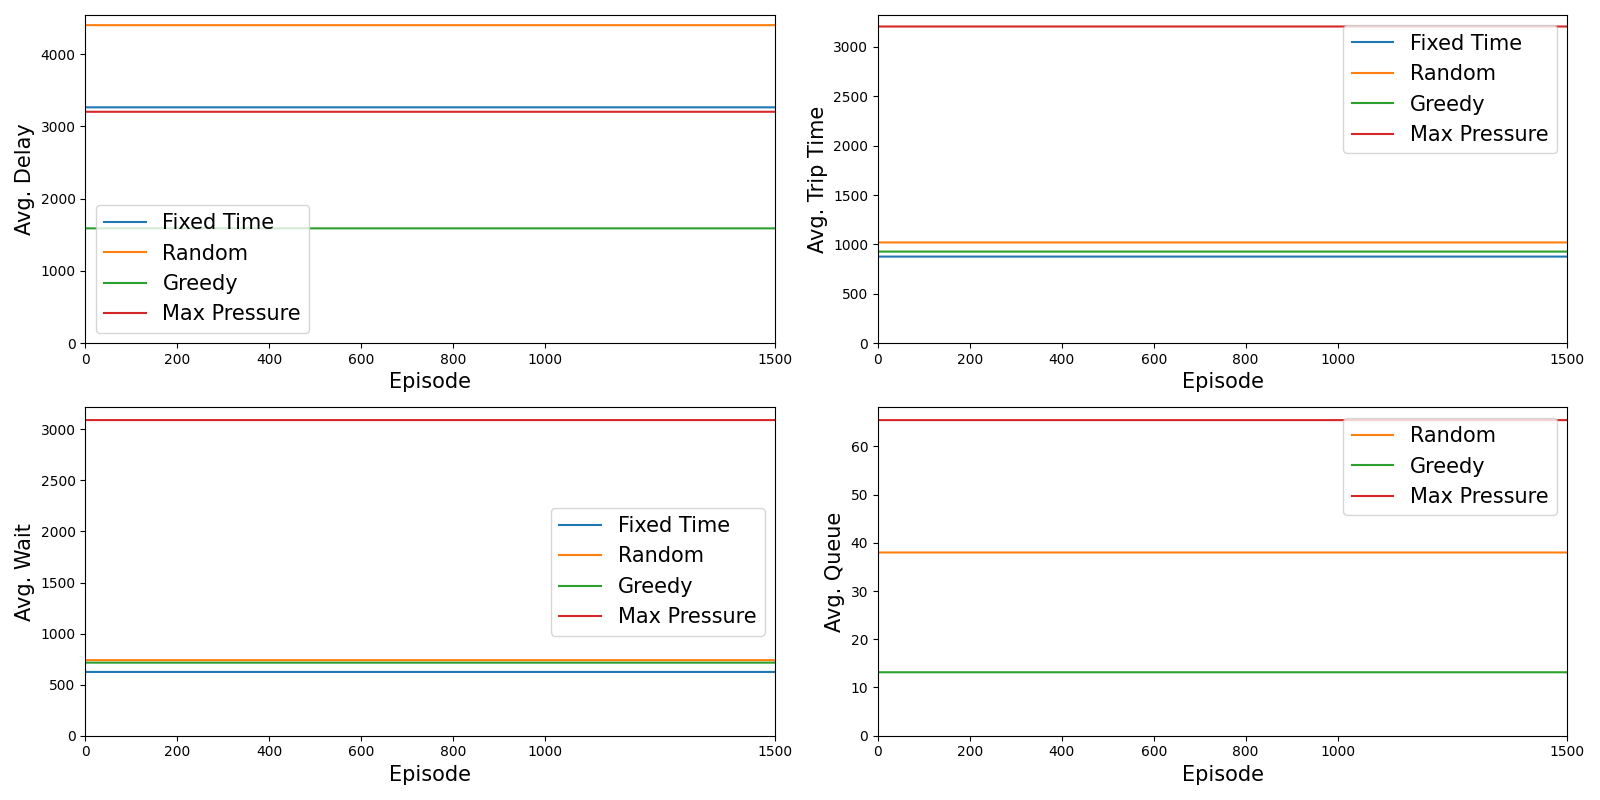
\includegraphics[width=1\linewidth]{images/experiments/baseline.png}
    \caption{Baseline Results}
    \label{fig:baseline_results}
\end{figure}

These baseline controllers play a pivotal role in our evaluation process, as they set the fundamental performance standards against which RL agents will be compared. Among the baseline controllers, particular attention is given to the Fixed Time Controller, as it closely emulates the real-world conditions of the target street.

Surprisingly, in certain scenarios, the Fixed Time Controller outperforms even the Max Wave and Max Pressure Agents. This phenomenon can be attributed to the highly optimized nature of Fixed Time control, which aims to provide a generalized solution across various traffic conditions. The baseline results, thus, offer valuable insights into the inherent challenges and complexities of traffic light control.

The comparison between our RL agents and these baseline controllers will shed light on the efficacy of reinforcement learning approaches in optimizing urban traffic flow.

\section{IDQN} \label{sec:exp-idqn}
The IDQN (Independent Deep Q-Network) agent is designed to utilize both state and reward representations to make informed traffic light control decisions. For state representation, we have chosen \hyperref[subsec:state-2]{State 2}, which encompasses critical attributes such as approach, total wait time, queue length, and total speed. This comprehensive state representation provides the agent with a wealth of observable information, facilitating intelligent decision-making.

Regarding the choice of reward, we have opted for \hyperref[subsec:reward-2]{Reward 2}, which represents the normalized total wait time. By using this reward metric, the agent aims to minimize the cumulative waiting time of vehicles at the intersection.

The observable range for traffic lights, which defines the distance at which they can detect approaching vehicles, is set at 200 meters.

The results section for the IDQN controller will provide an in-depth analysis of the controller's performance in terms of various metrics, including average delay, wait times, queue lengths, and trip times. These results will be essential for evaluating the effectiveness of the IDQN agent in optimizing traffic light control.

\subsection{Results}
Let's begin by examining the outcomes obtained from the IDQN RL Controller. The results are illustrated in Figure \ref{fig:idqn_results} below:

\begin{figure}[h]
    \centering
    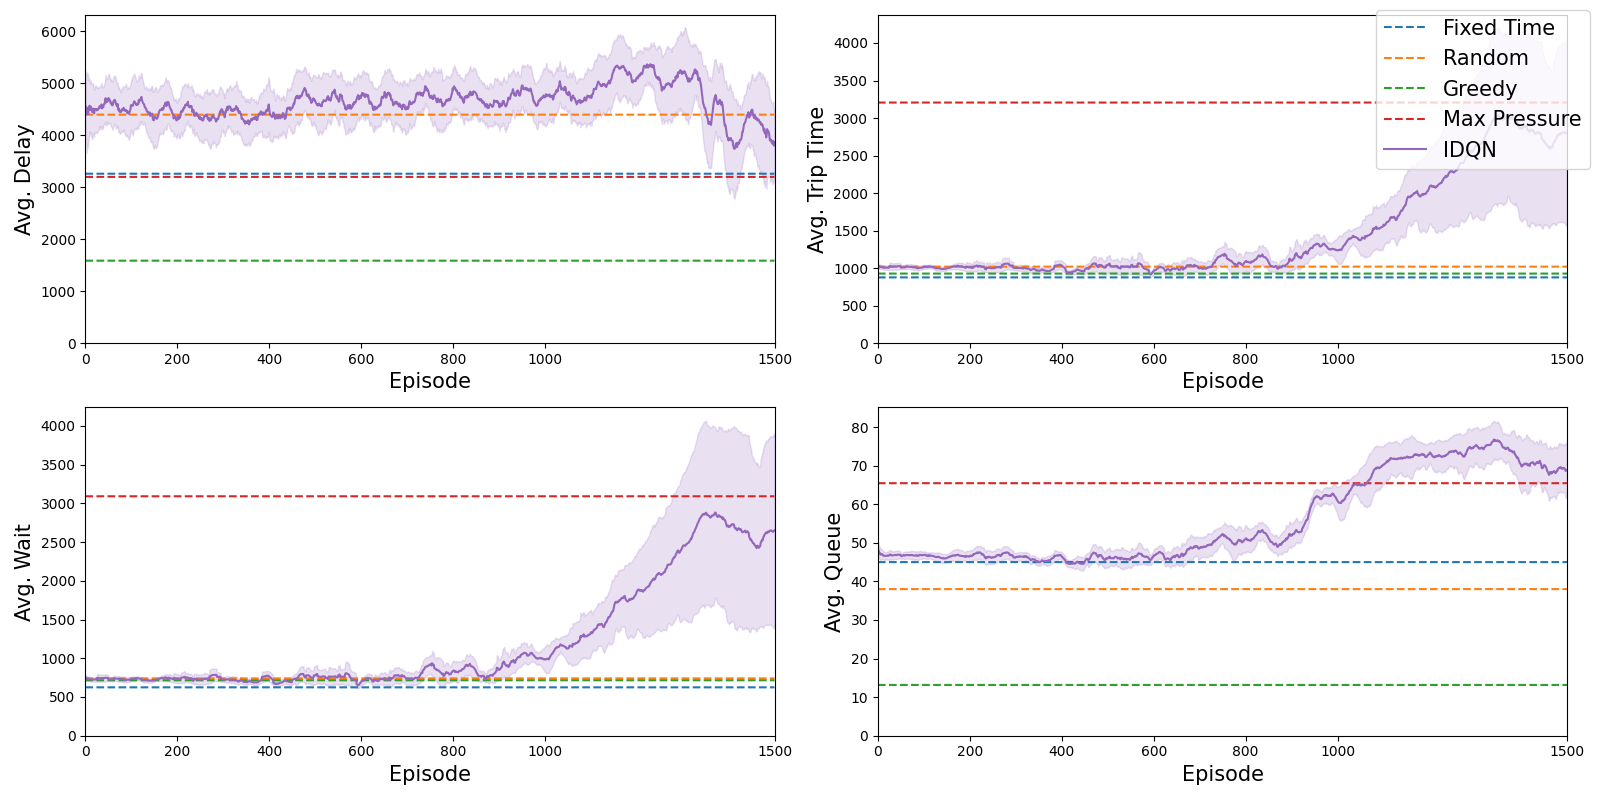
\includegraphics[width=1\linewidth]{images/experiments/IDQN.png}
    \caption{IDQN Performance Compared to Baselines}
    \label{fig:idqn_results}
\end{figure}

In Figure \ref{fig:idqn_results}, we present the performance of the IDQN agent across four key metrics: Average Delay, Average Trip Time, Average Wait, and Average Queue. Analyzing these metrics in the context of this specific map, we observe that the IDQN agent did not outperform the Random Baseline Controller.

Considering that the reward function used for IDQN was \hyperref[subsec:reward-2]{Reward 2} and for state representation we used \hyperref[subsec:state-2]{State 2}, which is based on minimizing waiting time, it is noteworthy that IDQN initially demonstrated promising results. During the initial stages, it performed comparably to the Fixed and Greedy Baseline Controllers. However, as the simulation progressed beyond 1000 episodes, its performance deteriorated.

In summary, the IDQN RL Controller did not prove to be an optimal solution for the given map and traffic control problem. The observed decline in performance raises questions about the suitability of the selected state and reward representations for this specific scenario.

\section{IPPO}
The IPPO controller shares the same state and reward representations as the \hyperref[sec:exp-idqn]{IDQN} agent. It utilizes \hyperref[subsec:state-2]{State 2}, which encapsulates approach, total wait time, queue length, and total speed, and \hyperref[subsec:reward-2]{Reward 2}, which normalizes the total wait time.

Similar to the IDQN agent, the maximum observable distance for traffic lights is set at 200 meters.

The results section for the IPPO controller will present an evaluation of its performance based on various metrics. These metrics will provide insights into the controller's ability to optimize traffic light control under real-world conditions.

\subsection{Results}
To begin, let's examine the results obtained from the IPPO RL Controller:

\begin{figure}[h]
    \centering
    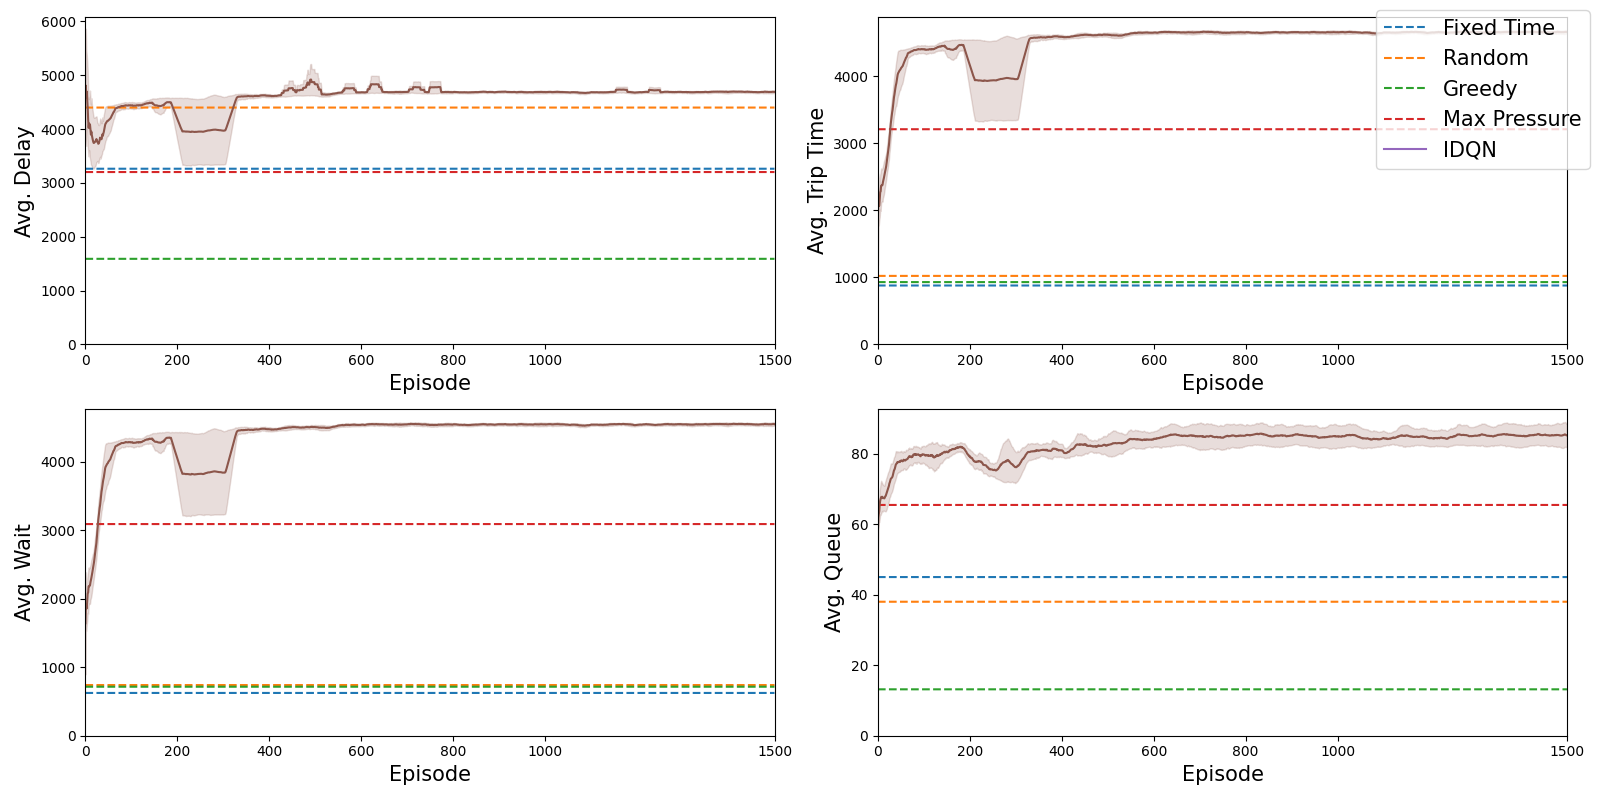
\includegraphics[width=1\linewidth]{images/experiments/IPPO.png}
    \caption{IPPO Performance Compared to Baselines}
    \label{fig:ippo_results}
\end{figure}

In Figure \ref{fig:ippo_results}, we present the performance of the IPPO agent across four critical metrics: Average Delay, Average Trip Time, Average Wait, and Average Queue. Upon analyzing these metrics within the context of this specific map, it becomes evident that the IPPO controller did not perform favorably, failing to surpass any of the baseline controllers.

In contrast to the IDQN controller, which showed promise initially, the IPPO agent faced difficulties right from the start and consistently performed poorly throughout the simulation. The state representation employed by IPPO, \hyperref[subsec:state-2]{State 2}, encompasses crucial attributes such as approach, total wait time, queue length, and total speed. Additionally, IPPO utilized \hyperref[subsec:reward-2]{Reward 2}, which normalizes the total wait time. However, even in the metric related to total wait time, IPPO exhibited subpar performance.

In summary, the IPPO RL Controller did not prove effective in managing the traffic flow within the given map. Its consistent underperformance across all metrics raises questions about its suitability for this specific traffic control scenario.

\section{MPLight} \label{sec:exp-mplight}
The MPLight (Max Pressure with Deep Reinforcement Learning for Traffic Signal Control) controller adopts a different state and reward representation strategy compared to the previous agents. For state representation, we employ \hyperref[subsec:state-3]{State 3}, which focuses solely on the pressure at the intersection. This simplified state representation centers the agent's attention on the critical factor of pressure.

The reward chosen for MPLight is \hyperref[subsec:reward-3]{Reward 3}, which is a negative value representing the queue length. This reward metric incentivizes the agent to minimize pressure and alleviate congestion.

Despite the change in state and reward representation, the observable range for traffic lights remains consistent at 200 meters.

The results section for the MPLight controller will provide an evaluation of its performance based on metrics related to queue length, delay, and other relevant factors. These results will help assess the effectiveness of MPLight in mitigating congestion at the intersection.

\subsection{Results} \label{sec:exp-mplight-results}
Let's begin by examining the results obtained from the MPLight RL Controller:

\begin{figure}[h]
    \centering
    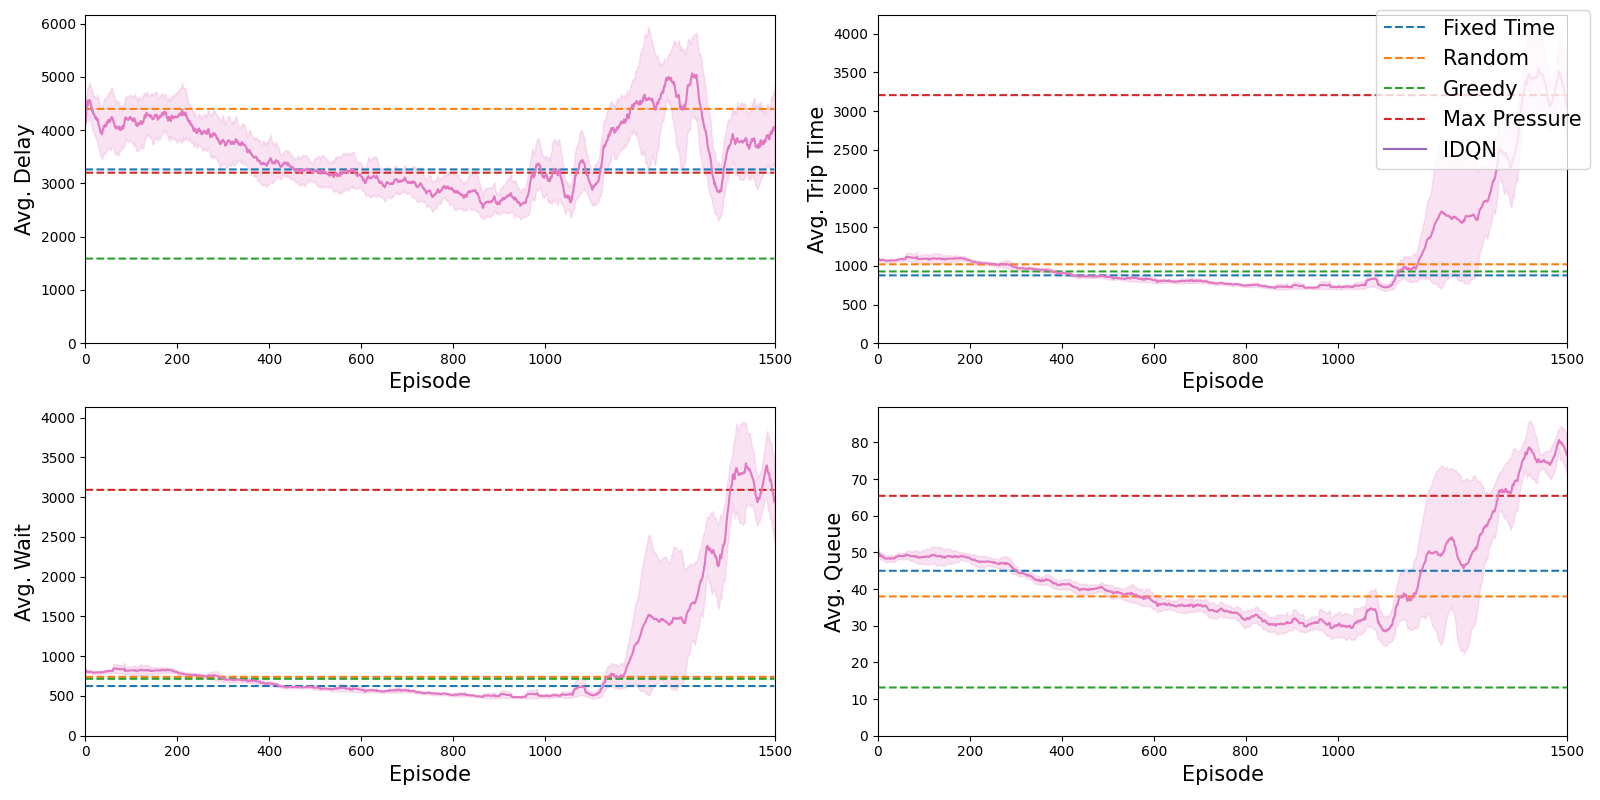
\includegraphics[width=1\linewidth]{images/experiments/MPLight.png}
    \caption{MPLight Performance Compared to Baselines}
    \label{fig:mplight_results}
\end{figure}

Figure \ref{fig:mplight_results} illustrates the performance of the MPLight agent across the same four essential metrics as the previous controllers: Average Delay, Average Trip Time, Average Wait, and Average Queue. Upon a detailed analysis of the results, it becomes evident that MPLight displayed a commendable performance overall.

In terms of Average Delay, MPLight managed to outperform all the baseline controllers, with the exception of the Greedy baseline, around the 800th episode. A similar trend can be observed in the Average Trip Time metric, where MPLight surpassed all controllers at approximately the same episode count. The story repeats itself when considering Average Wait Time, as MPLight excelled in performance around the same episode range.

Regarding Average Queue, MPLight reached its peak performance at around the 1250th episode, once again surpassing all baseline controllers except the Greedy baseline. Notably, MPLight relies on \hyperref[subsec:state-3]{State 3} and \hyperref[subsec:reward-3]{Reward 3}, which predominantly focuses on managing traffic pressure.

In summary, MPLight demonstrated an impressive ability to optimize traffic flow in the given scenario. While it may not have achieved significantly superior performance compared to baseline controllers, these results suggest that there is potential for further refinement and enhancement in its traffic control capabilities.

\section{MPLightFull}
MPLightFull is an extension of the \hyperref[sec:exp-mplight]{MPLight} controller. It employs a more comprehensive state representation, \hyperref[subsec:state-4]{State 4}, which includes queue length, normalized total wait time, total speed, and normalized approach. This richer state representation enables the agent to consider a broader range of factors when making traffic light control decisions.

The reward for MPLightFull remains the same as \hyperref[subsec:reward-3]{Reward 3}, emphasizing the reduction of pressure as the primary objective.

Like its predecessor, MPLightFull operates with an observable range of 200 meters for traffic lights.

The results section for the MPLightFull controller will provide an evaluation of its performance based on the chosen state and reward representations. Metrics related to queue length, delay, and other relevant aspects will be analyzed to determine the controller's effectiveness in optimizing traffic flow.

\subsection{Results}
Let's begin by examining the results obtained from the MPLightFull RL Controller:

\begin{figure}[h]
    \centering
    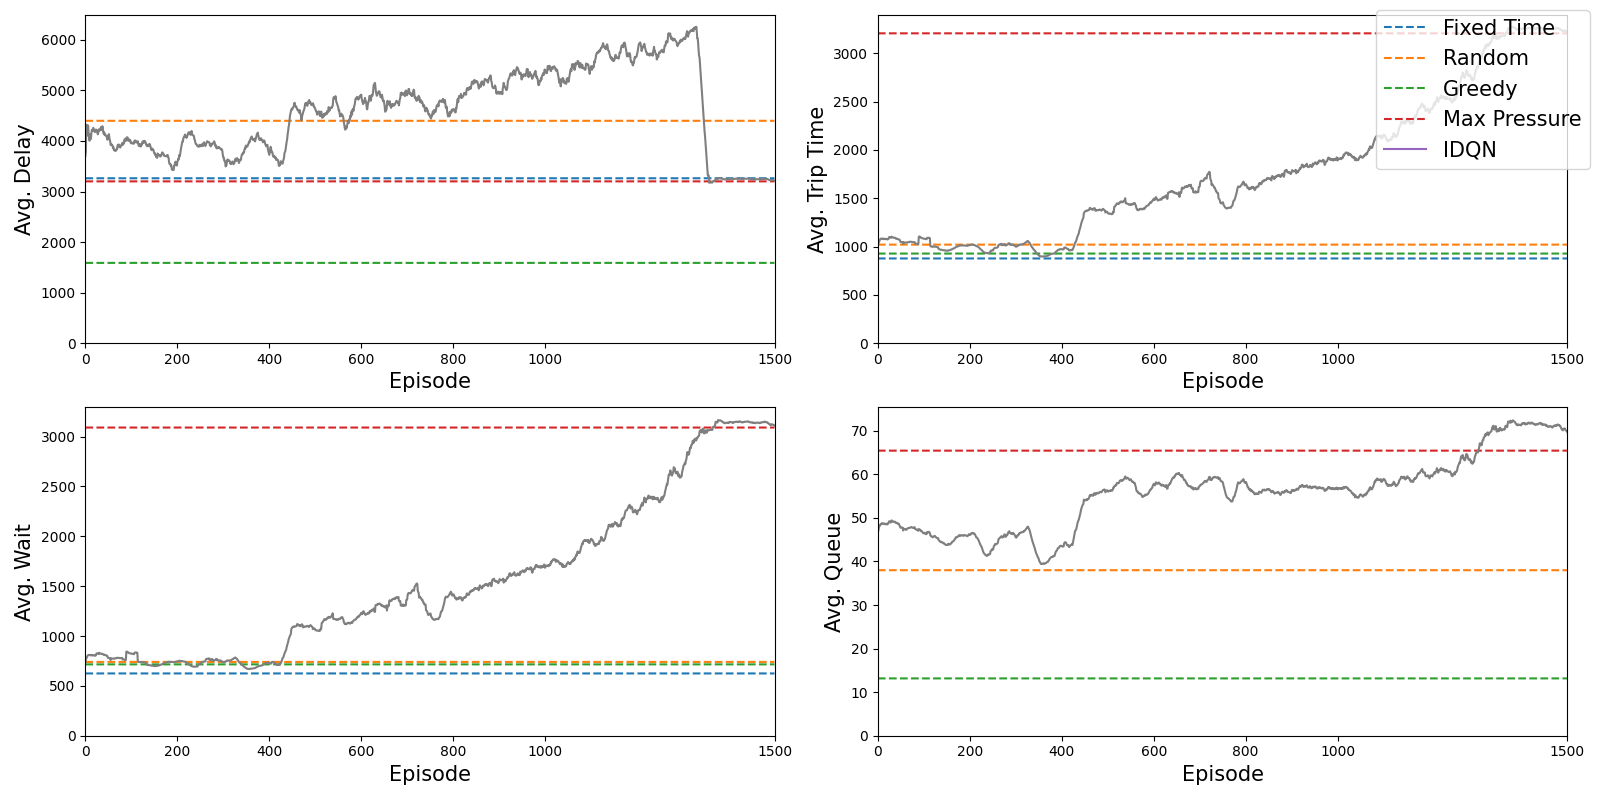
\includegraphics[width=1\linewidth]{images/experiments/MPLightFULL.png}
    \caption{MPLightFull Performance Compared to Baselines}
    \label{fig:mplightfull_results}
\end{figure}

In Figure \ref{fig:mplightfull_results}, we observe the results of the MPLightFull RL Controller across the same four fundamental metrics: Average Delay, Average Trip Time, Average Wait, and Average Queue, just as with the other controllers. It's intriguing to note that these results present an unexpected outcome.

Considering that the previous \hyperref[sec:exp-mplight-results]{MPLight Controller Results} displayed reasonably good performance, one might naturally expect that providing more extensive state representation through \hyperref[subsec:state-4]{State 4} would yield even better results. However, the reality turned out to be quite the opposite. MPLightFull's performance, in fact, deteriorated in all metrics, and in some cases, it struggled to outperform the Random Baseline controller.

This outcome emphasizes a crucial point: an abundance of state representation and additional information does not necessarily translate into improved performance. MPLightFull's performance serves as a clear illustration of this phenomenon.

In summary, the MPLightFull RL Controller's results demonstrate that more extensive state representation alone does not guarantee superior performance and may even lead to unexpected outcomes.

\section{FMA2C} \label{sec:exp-fma2c}
The FMA2C controller is a multi-agent system that employs specific state and reward representations tailored to its collaborative nature. For state representation, FMA2C uses \hyperref[subsec:state-6]{State 6}, which is customized to meet the requirements of multi-agent traffic control. This state representation is primarily based on approach and queue length, essential for coordinating traffic light control among multiple agents.

The reward used in FMA2C is a combined reward metric found under \hyperref[subsec:reward-4]{Reward 4}. This reward considers various factors, including departures, arrivals, the number of vehicles, queue length, and maximum wait time. It facilitates cooperative decision-making among agents.

The observable distance for traffic lights in FMA2C is set at 200 meters.

The results section for the FMA2C controller will provide a comprehensive evaluation of its performance in a multi-agent traffic control scenario. Metrics related to queue length, delay, and the collaborative behavior of the agents will be analyzed to assess the effectiveness of this multi-agent approach.

\subsection{Results}
Let's begin by examining the results obtained from the FMA2C RL Controller:

\begin{figure}[h]
    \centering
    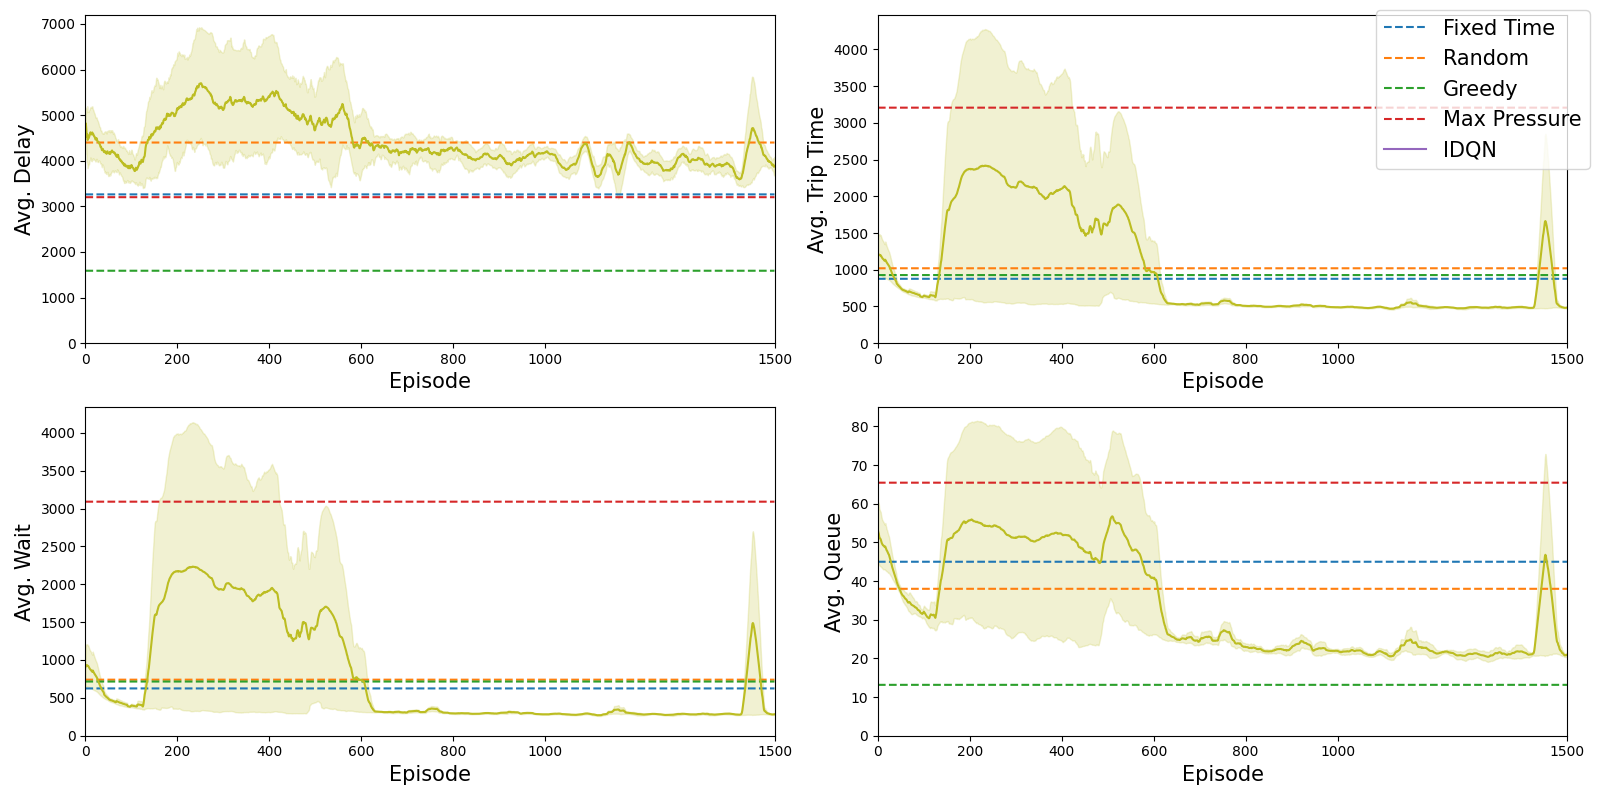
\includegraphics[width=1\linewidth]{images/experiments/FMA2C.png}
    \caption{FMA2C Performance Compared to Baselines}
    \label{fig:fama2c_results}
\end{figure}

In Figure \ref{fig:fama2c_results}, we can observe the results of the FMA2C RL Controller across the same four crucial metrics: Average Delay, Average Trip Time, Average Wait, and Average Queue, just as with the other controllers. It's important to note that the FMA2C Controller operates using a multi-agent control system.

When analyzing the Average Delay metric, we find that FMA2C did not excel during any phase of the training period. It mostly outperformed random controllers but struggled to compete with other baseline controllers. However, the standout performance of FMA2C is evident in both Average Trip Time and Average Wait Time metrics. These metrics share similarities due to their nature, and FMA2C demonstrated impressive results, surpassing all other controllers by a significant margin, with only a minor peak in performance around episode 500. Throughout training, it maintained a stable and noteworthy performance trajectory.

In the context of Average Queue, the pattern remains consistent, with a noticeable peak around episode 500 and overall stable progress. FMA2C significantly outperformed all other baseline controllers, with the exception of the greedy controller.

In summary, the FMA2C RL Controller exhibited remarkable performance results for this specific map and problem, particularly excelling in Average Trip Time and Average Wait Time metrics. These results underscore the effectiveness of the multi-agent control system employed by FMA2C in optimizing traffic flow.

\section{FMA2CFull}
FMA2CFull extends the capabilities of the \hyperref[sec:exp-fma2c]{FMA2C} controller by incorporating a more comprehensive state representation, \hyperref[subsec:state-7]{State 7}. This state representation includes additional parameters such as total wait time, the number of vehicles, and speed, providing a more detailed view of the traffic conditions.

The reward for FMA2CFull remains consistent with \hyperref[subsec:reward-5]{Reward 5}, which considers departures, arrivals, the number of vehicles, queue length, and maximum wait time.

The observable distance for traffic lights in FMA2CFull is set at 200 meters, aligning with the other controllers.

The results section for the FMA2CFull controller will evaluate its performance based on the extended state and reward representations. Metrics related to traffic flow, cooperative behavior among agents, and overall system efficiency will be analyzed to assess the advantages of this enhanced multi-agent approach.

\subsection{Results}
Let's begin by examining the results obtained from the FMA2CFull RL Controller:

\begin{figure}[h]
    \centering
    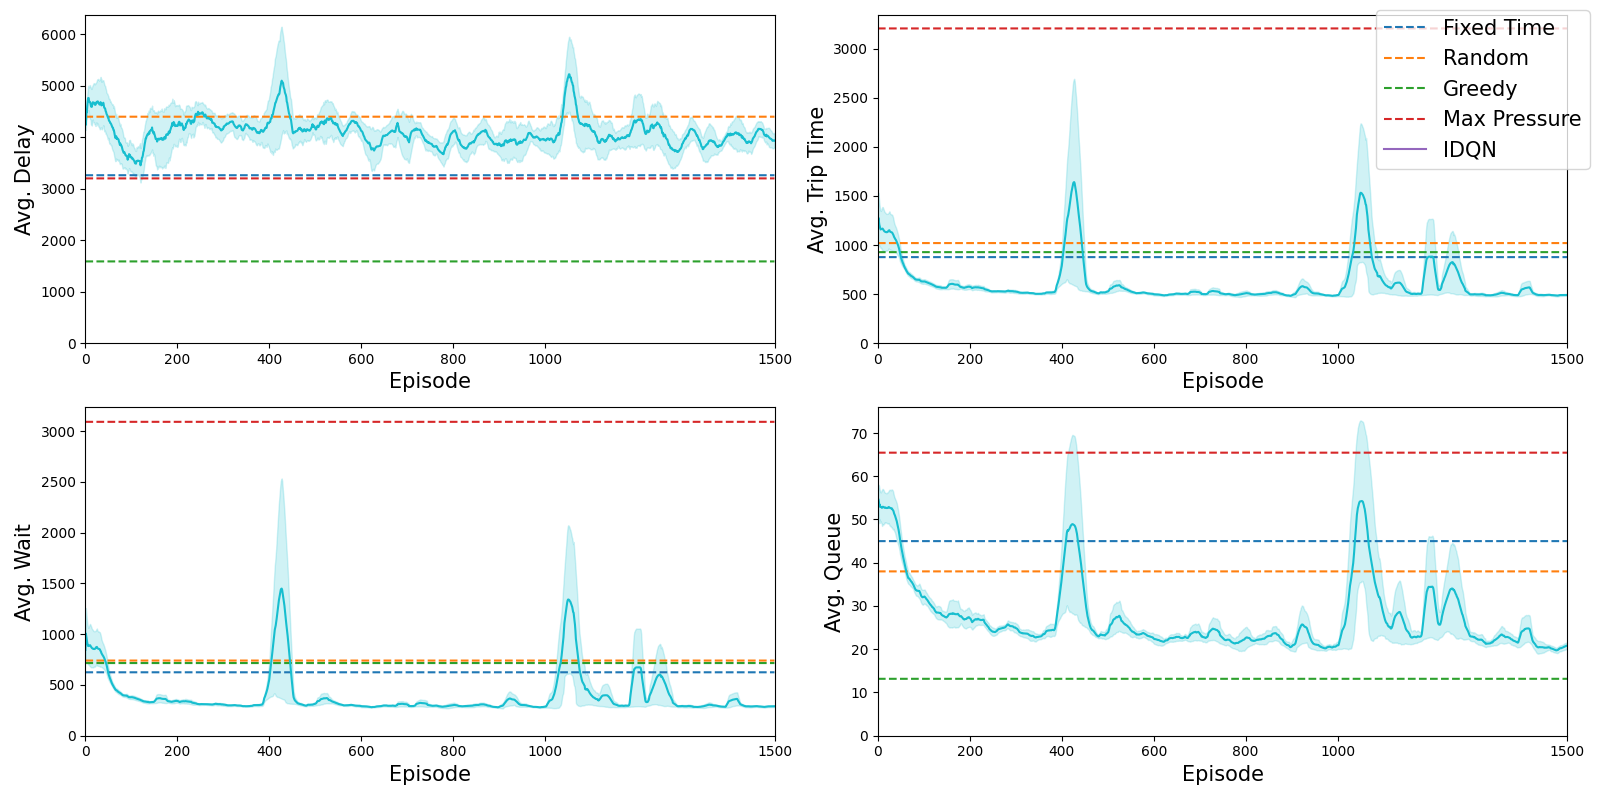
\includegraphics[width=1\linewidth]{images/experiments/FMA2CFULL.png}
    \caption{FMA2CFull Performance Compared to Baselines}
    \label{fig:fama2cfull_results}
\end{figure}

In Figure \ref{fig:fama2cfull_results}, we can observe the results of the FMA2CFull RL Controller across the same four essential metrics: Average Delay, Average Trip Time, Average Wait, and Average Queue, consistent with the other controllers. Similar to the situations with MPLight and MPLightFull, this controller aims to increase the information available to the agent by altering the state representation and employing \hyperref[subsec:state-7]{State 7}.

In contrast to the previous case with MPLightFull, the extended state representation of FMA2CFull did not significantly deteriorate or enhance the agent's performance. It maintained a comparable performance level throughout the training process. Specifically, in the Average Delay metric, FMA2CFull exhibited similar performance to only the random controller. However, it notably outperformed other baseline controllers in both Average Wait and Average Trip Time metrics. In terms of the Average Queue metric, FMA2CFull significantly outperformed all baseline controllers, except for the Greedy controller. Notably, the performance curves and progress of FMA2CFull mirrored those of MPLight but with a peak occurring around episode 1000 rather than episode 500.

To summarize, the introduction of an extended state representation did not substantially alter the overall performance of FMA2CFull. It maintained a level of performance similar to its predecessor and continued to excel in Average Wait and Average Trip Time metrics while significantly outperforming baseline controllers in Average Queue.

\section{Comparison}
\subsection{Controller Performance Comparison}
In this section, we will provide a comprehensive comparison of the various controllers used in our experiments. To facilitate this comparison, we present the combined results of all controllers in Figure \ref{fig:all_results}.

\begin{figure}[h]
    \centering
    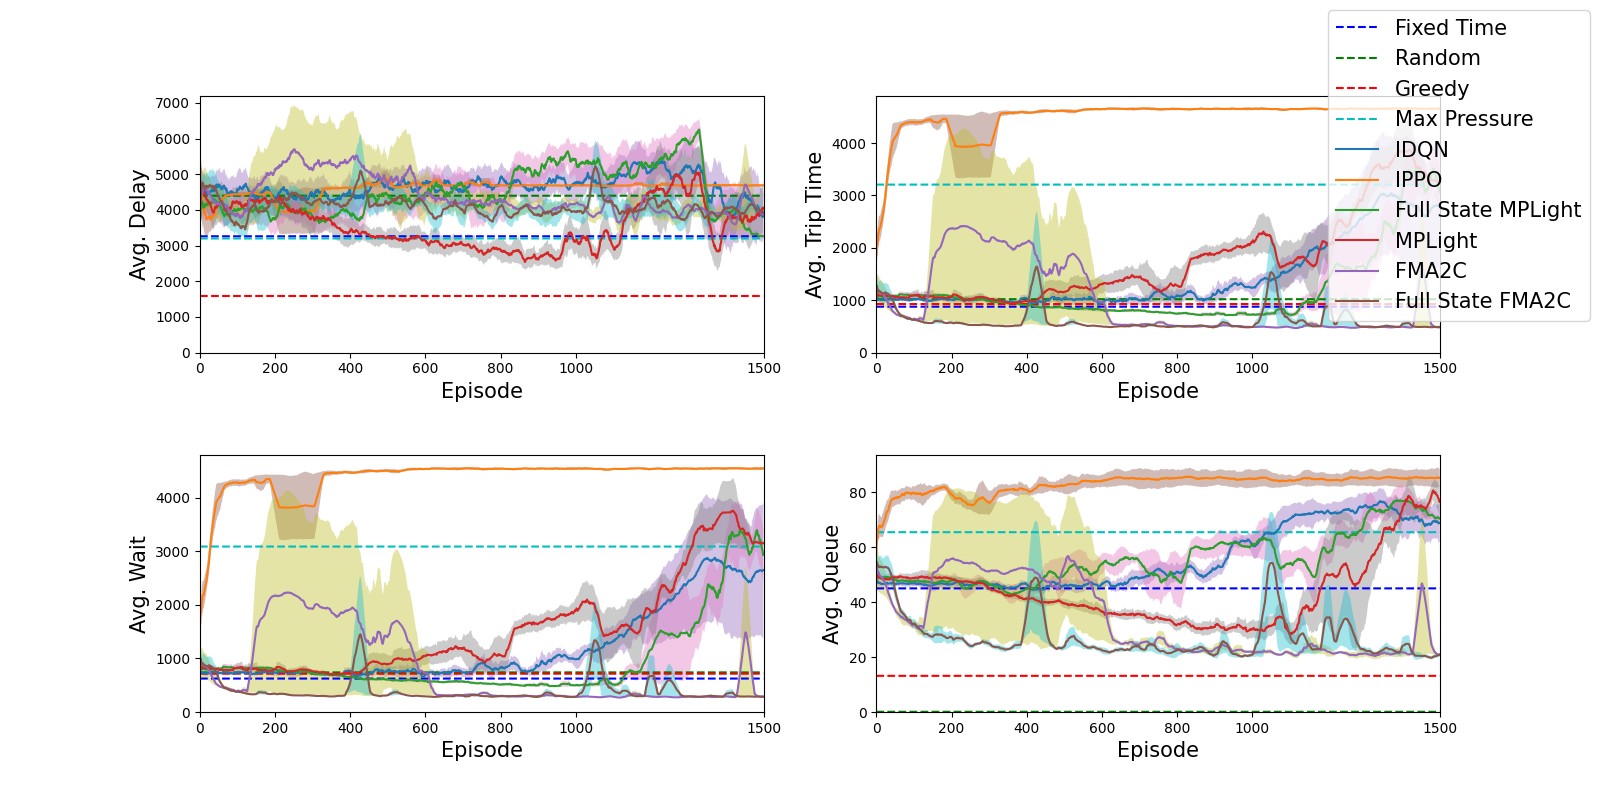
\includegraphics[width=1\linewidth]{images/experiments/all.png}
    \caption{Combined Performance Results of All Controllers}
    \label{fig:all_results}
\end{figure}
\newpage
Upon initial observation, Figure \ref{fig:all_results} may appear dense due to the simultaneous presence of multiple controllers. However, several noteworthy insights can be gleaned from this comprehensive overview. Let's delve into a few key observations:

1. \textbf{Average Delay:} In the context of Average Delay, MPLight stands out as a strong performer, surpassing all RL Controllers. Nevertheless, it falls short of outperforming the Greedy Controller, which excels in minimizing delay.

2. \textbf{Average Trip Time and Average Wait:} FMA2C and FMA2CFull controllers exhibit parallel performance trends in both Average Trip Time and Average Wait metrics. Following closely behind, MPLight maintains a competitive performance in these two crucial categories.

3. \textbf{Average Queue:} Similar to the Average Trip Time and Average Wait metrics, the performance of MPLight, FMA2C, and FMA2CFull aligns in terms of Average Queue management. These RL Controllers showcase impressive results compared to baseline controllers.

Overall, the comparative analysis of these controllers reveals nuanced performance patterns across various metrics. Each controller exhibits strengths in specific areas, highlighting the importance of selecting an appropriate controller based on the desired traffic management objective. The results underscore the potential of RL-based traffic light control methods to significantly improve urban traffic flow, with each controller contributing unique insights and performance nuances.

\subsection{Performance Summary Tables}

In this section, we provide a summary of the best performance achieved by each controller during training. Table \ref{tab:performance_comparison} presents a comprehensive comparison of baseline and RL controllers across four key metrics: Average Delay, Average Trip Time, Average Wait, and Average Queue.

\begin{table}[h]
    \centering
    \caption{Performance Comparison of Baseline and RL Controllers}
    \label{tab:performance_comparison}
    \begin{tabular}{|lcccc|}
        \hline
        \textbf{Controller} & \textbf{Avg. Delay} & \textbf{Avg. Trip Time} & \textbf{Avg. Wait} & \textbf{Avg. Queue} \\ \hline
        \textbf{Baseline Controllers} & & & & \\ \hline
        FIXED       
        & 3262.59                   
        & \textbf{877.08} 
        & \textbf{624.55} 
        & - \\
        STOCHASTIC  
        & 4399.18                   
        & 1020.2 
        & 740.09 
        & 38.2 \\
        MAXWAVE     
        & \textbf{\textit{1588.78}} 
        & 927.81 
        & 715.55 
        & \textbf{\textit{13.16}} \\
        MAXPRESSURE 
        & 3201.23                   
        & 3206.6 
        & 3090.56 
        & 65.45 \\ \hline
        \textbf{RL Controllers} & & & & \\ \hline
        IDQN        
        & 3993.99                   
        & 891.26 
        & 623.70 
        & 43.22 \\
        IPPO        
        & 3322.71                   
        & 1183.85 
        & 896.15 
        & 51.80 \\
        MPLight     
        & \textbf{2395.64}          
        & 705.73 
        & 480.66 
        & 22.09 \\
        MPLightFULL 
        & 3172.69                   
        & 896.91 
        & 669.03 
        & 39.42 \\
        \textbf{FMA2C}       
        & 3475.60                   
        & \textbf{\textit{471.83}} 
        & \textbf{\textit{272.02}} 
        & \textbf{19.11} \\
        FMA2CFULL   
        & 3345.40                   
        & 477.61 
        & 277.39 
        & 19.24 \\ \hline
    \end{tabular}
\end{table}

\newpage
In Table \ref{tab:performance_comparison}, we have categorized controllers into two groups: baseline and RL controllers. Within each category, the best-performing metric is bolded, and for the absolute best within that metric, we have used both bold and italic formatting.

For Average Delay, the MAXWAVE baseline controller exhibited the best performance, while among RL controllers, MPLight achieved the lowest delay. However, MAXWAVE outperformed MPLight in this metric, indicating that RL did not significantly improve this aspect.

In terms of Average Trip Time, the FIXED baseline controller and FMA2C RL controller displayed the best results, with FMA2C outperforming the others by almost twice the performance.

For Average Wait, the same pattern as Average Trip Time emerged, with FIXED and FMA2C leading the way. Here, FMA2C achieved more than double the performance of other controllers in the RL category.

In the Average Queue metric, MAXWAVE and FMA2C performed well, with MAXWAVE having a 50\% lead over FMA2C.

Considering the overall results, the RL controller FMA2C consistently outperforms other RL controllers in three out of four metrics, making it a promising choice for this traffic management scenario.

\subsection{Comparison with RESCO Results}

In this section, we will compare our experimental results with those from RESCO (\cite{resco}). First, let's examine their findings presented in Figure \ref{fig:resco_results}.

\begin{figure}[h]
    \centering
    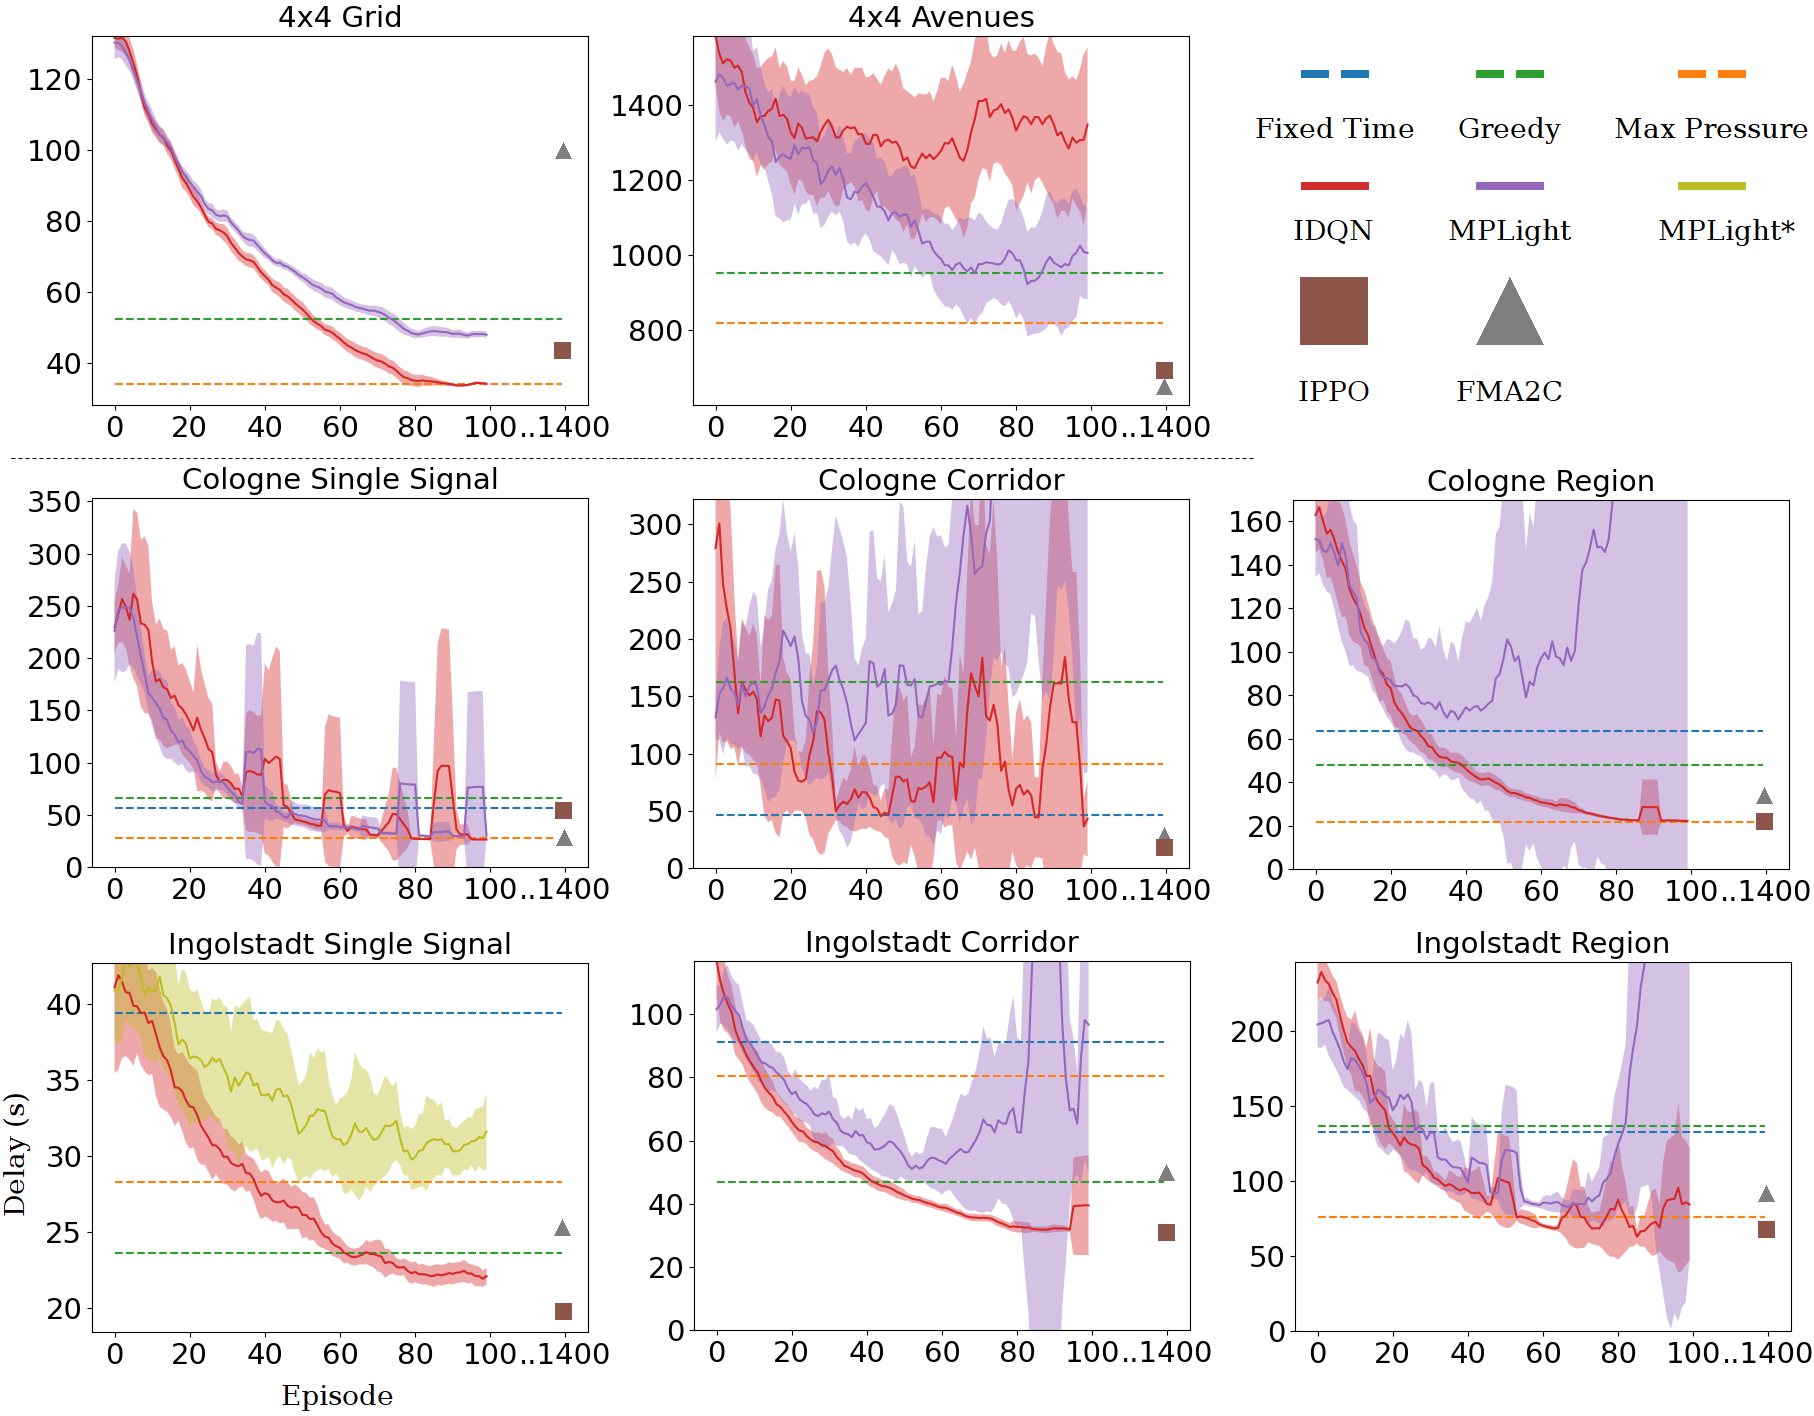
\includegraphics[width=1\linewidth]{images/experiments/delays.png}
    \caption{RESCO Results\cite{resco}}
    \label{fig:resco_results}
\end{figure}

\newpage

From RESCO's results, it is evident that IPPO and FMA2C performed exceptionally well. However, when we compare these results to our own experiments, the performance of IPPO was notably worse in our case, and only FMA2C demonstrated strong performance, consistently outperforming other controllers in our experiments.

It's crucial to note that RESCO's experiments encompassed various maps, and while their RL controllers excelled in almost all scenarios, the specific performance and progress can vary significantly depending on the map. This highlights the importance of tailoring RL models to the unique challenges presented by each map. Different maps may demand different strategies, and a one-size-fits-all approach is unlikely to yield optimal results.

In conclusion, our experiments align with RESCO's findings in terms of FMA2C's strong performance. However, the discrepancy in IPPO's performance underscores the need for map-specific research and the careful selection of RL models to address the distinct challenges posed by different maps.
